% Sone family preprint. Build with `make` (tectonic main.tex).
\documentclass[11pt]{article}

\usepackage[T1]{fontenc}
\usepackage{lmodern}
\usepackage[a4paper,margin=0.95in]{geometry}
\usepackage{amsmath,amssymb}
\usepackage{booktabs}
\usepackage{graphicx}
\usepackage{subcaption}
\usepackage{placeins}
\usepackage{xcolor}
\usepackage{microtype}
\usepackage{algorithm}
\usepackage{algpseudocode}
\usepackage{listings}
\usepackage[numbers,sort&compress]{natbib}
\usepackage[colorlinks=true,linkcolor=blue!50!black,citecolor=blue!50!black,urlcolor=blue!50!black]{hyperref}

\newcommand{\sone}{Sone}
\newcommand{\op}[1]{\texttt{#1}}
\newcommand{\R}{\mathbb{R}}
\DeclareMathOperator*{\argmin}{arg\,min}
\lstset{basicstyle=\ttfamily\footnotesize,breaklines=true,columns=fullflexible,frame=single,framesep=4pt,xleftmargin=4pt,xrightmargin=4pt,upquote=true}

\title{\textbf{Sone}: Sub-Core CPU DJ Transitions via Phase-Coherent Tonotopic Separation, Equivariant Metrical Perception, and Cortical Planning}
\author{Luka L\"ohr\\Independent Researcher}
\date{}

\begin{document}
\emergencystretch=1.5em
\maketitle

\begin{abstract}
Continuous music radio and personalised playlist playback require beat-locked, harmonically clean transitions between arbitrary stereo recordings without altering studio masters outside the blend or maintaining GPU servers per stream. End-to-end generative audio codecs degrade non-transition audio, introduce phase-scrambled vocal artifacts on dense mixes, and exceed single-core CPU budgets by orders of magnitude. We present \textbf{\sone{}}, a three-tier family of unified neuro-symbolic automatic DJ models---\textbf{Sone-6.5M} ($13.12$\,MB FP16), \textbf{Sone-v2-Base} ($13.61$\,M parameters, $27.36$\,MB), and \textbf{Sone-Pro} ($26.37$\,M parameters, $52.90$\,MB)---built on a strict separation of responsibilities: four neural organs modelled after the human auditory-to-executive pathway and packaged inside a single \op{model.safetensors} file \emph{separate, perceive, plan, and monitor} transitions exclusively within a $\sim 24$\,s boundary window, while a deterministic Rust DSP engine executes phase-locked time-stretching, vocal-pocket mixing, and raised-cosine splicing into untouched master stereo outside the transition. Specifically, \sone{} integrates (i) \textbf{Cochlea} (\op{cochlea.*}), scaled in \op{v2/Pro} to a $4096$-point STFT ($10.77$\,Hz resolution), $64$ vocal-harmonic subbands, Dual-Axis Time+Band Transformers, and bounded complex masks projected onto exact mixture consistency ($\|\sum_{m=1}^4 \hat{s}_m - x\|_\infty < -148$\,dB) under active-vocal cosine phase-coherence, $128$-mel perceptual, and bidirectional anti-bleed losses distilled from \op{HTDemucs-ft} over $1{,}101$ Creative Commons tracks plus MUSDB18-HQ ($7.84$\,dB held-out vocal SDR at $0.95\times$ 1-vCPU real-time); (ii) \textbf{Tympanum} (\op{tympanum.*}), a $50$\,Hz dilated TCN--BiGRU trained with exact vinyl-speed pitch/key/tuning/tempo equivariance and paired with a neuro-symbolic multi-octave comb-grid tracker ($12/12$ exact BPM locks); (iii) \textbf{Cortex} (\op{cortex.*}), an $8$-layer beat-synchronous Transformer predicting recipes, bar offsets ($0.165$\,bar held-out MAE), and eight stem gain trajectories ($0.0170$ MAE); and (iv) \textbf{Cingulate} (\op{cingulate.*}), a $6$-layer conflict Transformer trained with $50\%$ on-GPU counterfactual DJ defect synthesis across $30$ defect classes ($97.00\%$ held-out accuracy) for Best-of-$K$ candidate reranking. Across four generations of NVIDIA Tensor Core GPUs (T4, L4, A100, and dual $96$\,GB RTX PRO 6000 Blackwell \op{sm\_120} accelerators) and a dependency-free single-threaded Rust/WebAssembly runtime (\op{sone-infer/1}), all three \sone{} tiers run faster than real-time on a single Intel Xeon vCPU ($4.8\%$--$27.1\%$ average core load per $3$\,min song) while lifting blind-tested vocal-handoff loudness floors by $+10.55$\,dB.
\end{abstract}

\section{Introduction}
\label{sec:intro}

A continuous music radio station or automated DJ player joins each outgoing track (Deck~A) to an incoming track (Deck~B) across a transition zone of four to sixteen bars. Executing a studio-grade transition requires aligning beats and downbeats to sub-$10$\,ms accuracy, matching tempo without shifting pitch, choosing an entry structure suited to both arrangements (such as layering Deck~B's opening vocals over Deck~A's instrumental groove or sneaking percussion under an outro), carving conflicting basslines and mid-range chords, and cutting outgoing vocals on a natural breath with a tempo-synced echo tail. Crucially, DJ mixing is a \emph{boundary} operation: for the remaining $85$--$90\%$ of every song outside the overlap $[u_0, u_1]$, listeners expect to hear the original studio master completely unaltered.

End-to-end generative audio models violate this structure in three ways. First, routing full songs through neural waveform or latent codecs degrades non-transition audio and introduces phase-scrambled, watery vocal artifacts on dense mixes. Second, generative audio backbones require hundreds of millions of parameters and dedicated GPUs, whereas streaming platforms serving thousands of concurrent personalised stations require transitions to render asynchronously on fractional cloud vCPUs or client-side WebAssembly workers. Third, DJ mixing is governed by discrete metrical and psychoacoustic invariants---bar phase, vocal onset locks, harmonic compatibility, and breath boundaries---where small regression smoothing errors create jarring perceptual defects even when average $L_1$ loss is low.

We take the opposite approach: \emph{perceive and plan with compact anatomical neural organs inside the boundary window; render and splice master audio with deterministic signal processing}. Outside $[u_0, u_1]$, \sone{} splices the untouched stereo master via raised-cosine seams and smooth post-handoff tempo glides, guaranteeing zero neural coloration on the body of every song and reducing per-track separation compute by $\sim 7.5\times$. Within the boundary window, four specialised neural organs packaged inside one unified \op{model.safetensors} checkpoint mirror the human auditory-to-executive pathway: \textbf{Cochlea} decomposes stereo mixtures into four phase-coherent stems, \textbf{Tympanum} extracts $50$\,Hz metrical and vocal-breath structure, \textbf{Cortex} plans beat-synchronous stem trajectories, and \textbf{Cingulate} monitors $30$ DJ conflict and defect modes~\citep{botvinick2001conflict} to rerank candidate plans. We name the model family \textbf{\sone{}} after Stevens' psychoacoustic unit of perceived loudness~\citep{stevens1936scale}, reflecting our core empirical finding that club-grade transitions hinge on perceived loudness continuity, vocal-formant phase coherence, and vocal-onset timing.

Scaling \sone{} across four generations of NVIDIA Tensor Core GPUs---from Turing (T4) and Ada Lovelace (L4) to Ampere (A100) and dual $96$\,GB Blackwell Server Edition (\op{sm\_120}) accelerators---allowed us to study both architectural and data scaling while preserving sub-core CPU deployability. In particular, upgrading \op{Cochlea} from a $2048$-point STFT ($21.5$\,Hz bin width) with unconstrained three-stem masking (\op{Sone-6.5M}) to a $4096$-point STFT ($10.77$\,Hz bin width), $64$ vocal-harmonic subbands, Dual-Axis Time+Band attention, bounded four-stem Wiener mixture projection, active-vocal cosine phase loss, and GPU teacher distillation over $1{,}101$ modern Creative Commons tracks (\op{Sone-v2-Base} and \op{Sone-Pro}) directly targets the phase scrambling and drum-hat bleed that plague lightweight separators. Likewise, training \op{Tympanum v2} with exact vinyl-speed pitch/tempo equivariance and coupling it at inference with a neuro-symbolic multi-octave comb-grid tracker eliminates octave tempo errors without Dynamic Bayesian Networks.

\paragraph{Contributions.}
\begin{itemize}
  \item \textbf{Three-tier unified neuro-symbolic DJ family (\S\ref{sec:method}):} \textbf{Sone-6.5M} ($6.52$\,M params, $13.12$\,MB FP16), \textbf{Sone-v2-Base} ($13.61$\,M, $27.36$\,MB), and \textbf{Sone-Pro} ($26.37$\,M, $52.90$\,MB), all sharing a single zero-copy Rust/WebAssembly wire format (\op{sone-infer/1}) and master-spliced boundary execution ($4.8\%$--$27.1\%$ of one Xeon vCPU per song).
  \item \textbf{Phase-coherent Dual-Axis \op{Cochlea} with teacher distillation (\S\ref{sec:stems}):} A $4096$-FFT, $64$-band Dual-Axis Time+Band Transformer with bounded complex masks ($2\tanh(M/2)$), stereo energy-weighted Wiener mixture projection ($\|\sum_m \hat{s}_m - x\|_\infty < -148$\,dB), active-vocal cosine phase loss, $128$-mel perceptual loss~\citep{yamamoto2020parallel}, and on-the-fly \op{HTDemucs-ft}~\citep{rouard2023hybrid} distillation across $1{,}101$ Creative Commons tracks~\citep{bogdanov2019mtg,manco2023song} plus MUSDB18-HQ~\citep{MUSDB18HQ}, lifting MUSDB18-HQ vocal SDR from $3.57$\,dB to $\mathbf{7.84}$\,\textbf{dB} ($5.55$\,dB mean SDR) at $0.95\times$ real-time on one CPU core.
  \item \textbf{Vinyl-speed equivariant \op{Tympanum} \& neuro-symbolic comb-grid (\S\ref{sec:ear}):} Exact pitch/key/tuning/tempo equivariant resampling ($\alpha = 2^{\Delta s/12}$) with zero timestamp drift across $600$ stem-isolated and modern tracks ($0.865$ raw beat F1, $0.506$ downbeat F1), fused with physical onset-flux F1 comb-grid period selection ($12/12$ exact BPM locks).
  \item \textbf{Cortical sharp-cut planning, $30$-defect counterfactual critique, and vocal-onset lock (\S\ref{sec:beat}):} Scaling \op{Cortex v3-Pro} ($8\text{L}/192\text{D}$, $0.165$\,bar held-out MAE, $0.0170$ lane MAE) and \op{Cingulate v3-Pro} ($6\text{L}/128\text{D}$, $50\%$ GPU counterfactuals, $97.00\%$ held-out accuracy) with Best-of-$K$ reranking and vocal-onset handoff ($+10.55$\,dB blend loudness floor).
  \item \textbf{Four-generation GPU \& single-core CPU systems audit (\S\ref{sec:experiments}--\S\ref{sec:results}):} Complete throughput, VRAM, and scaling measurements across NVIDIA T4, L4, A100, and $96$\,GB RTX PRO 6000 Blackwell GPUs alongside bit-accurate FP32-vs-FP16 Rust parity ($\le 2.39\times 10^{-4}$ max waveform diff).
\end{itemize}

\section{Related Work}
\label{sec:related}

\paragraph{Music source separation and knowledge distillation.}
Four-stem separation (\op{vocals}, \op{drums}, \op{bass}, \op{other}) on uncompressed benchmarks such as MUSDB18-HQ~\citep{MUSDB18HQ} and the Sound Demixing Challenge (MDX23)~\citep{fabbro2024sdx} is led by hybrid time--frequency transformers (HTDemucs)~\citep{rouard2023hybrid} and psychoacoustic band-split architectures including Band-Split RNN (BSRNN)~\citep{luo2023music} and BS-RoFormer~\citep{lu2024bsroformer}. While studio ensembles achieve strong signal-to-distortion ratios (SDR)~\citep{vincent2006performance}, their memory footprints and multi-second GPU runtimes preclude per-stream CPU radio deployment. Conversely, naively shrinking $2048$-point STFT separators degrades vocal harmonic spacing ($21.5$\,Hz/bin blurs low fundamental formants and vibrato) and produces phase-incoherent ``watery'' vocals when unconstrained masks cancel across stems. \sone{} bridges offline studio teachers and sub-core CPU inference via knowledge distillation~\citep{hinton2015distilling}: we run \op{HTDemucs-ft}~\citep{rouard2023hybrid} in $96$\,GB GPU memory over Creative Commons corpora (MTG-Jamendo~\citep{bogdanov2019mtg} and Song Describer~\citep{manco2023song}) to supervise a $4096$-FFT ($10.77$\,Hz/bin), $64$-band Dual-Axis Transformer equipped with bounded complex masks, exact energy-weighted Wiener mixture projection, multi-resolution STFT + $128$-mel perceptual loss~\citep{yamamoto2020parallel}, and explicit vocal cosine phase regularisation.

\paragraph{Metrical, vocal, and harmonic music analysis.}
Joint beat and downbeat tracking with temporal convolutional networks (TCNs) and bidirectional recurrent layers was established by \citet{bock2020deconstruct}, and \citet{foscarin2024beat} demonstrated with \emph{Beat This!} that shift-tolerant supervision can eliminate Dynamic Bayesian Network (DBN) post-processing. Automatic DJ planning, however, simultaneously requires frame-accurate active singing, singer breath boundaries ($\ge 0.28$\,s inter-line pauses for echo throws), eight-bar structural downbeats, $24$-class major/minor key, and concert-pitch tuning offsets (cents). Because public seven-head datasets are small ($<200$ songs), baseline TCN--BiGRUs quickly memorise track keys and tempos. Our \op{Tympanum v2} resolves data scarcity through exact vinyl-speed equivariant resampling---simultaneously transforming pitch class, sub-semitone tuning, and all five temporal event streams with zero label drift---and pairs neural $50$\,Hz activations at inference with a deterministic multi-octave comb-grid tracker over physical spectral flux.

\paragraph{Automatic DJ transitions.}
Rule-based automatic DJ systems progress from beat-matched crossfading~\citep{cliff2000hang} and playlist transition point selection~\citep{bittner2017automatic} to genre-specific drum-and-bass engines~\citep{vandeveire2018raw}. While deterministic templates preserve audio quality and bar lock, fixed fader curves cannot adapt to arbitrary vocal intros or audit harmonic clashes. Learning-based differentiable DJ mixers with adversarial waveform critics~\citep{chen2022automatic} demonstrate learned fader/EQ control, yet GAN objectives struggle to enforce discrete DJ invariants such as never cutting a vocalist mid-syllable or dimming accompaniment prior to incoming audio. Inspired by cognitive conflict monitoring in the anterior cingulate cortex~\citep{botvinick2001conflict}, \sone{} pairs an executive Beat Transformer (\op{Cortex}) with a $30$-defect counterfactual judge (\op{Cingulate}) for Best-of-$K$ plan selection, wrapped around vocal-onset-locked DSP rendering and untouched master splicing.

\section{Method}
\label{sec:method}

Figure~\ref{fig:architecture} illustrates the complete \sone{} architecture, and Table~\ref{tab:params} details exact tensor counts, parameter counts, and serialized FP16 footprints across \textbf{Sone-6.5M}, \textbf{Sone-v2-Base}, and \textbf{Sone-Pro}. We formalise the bar-ruler representation and untouched master splicing (\S\ref{sec:ruler}), derive phase-coherent Dual-Axis \op{Cochlea} (\S\ref{sec:stems}), vinyl-speed equivariant \op{Tympanum} and neuro-symbolic comb-grid tracking (\S\ref{sec:ear}), \op{Cortex} and \op{Cingulate} with Best-of-$K$ reranking and vocal-onset lock (\S\ref{sec:beat}), and the zero-copy Rust/WebAssembly runtime (\S\ref{sec:runtime}).

\begin{figure*}[!tbp]
  \centering
  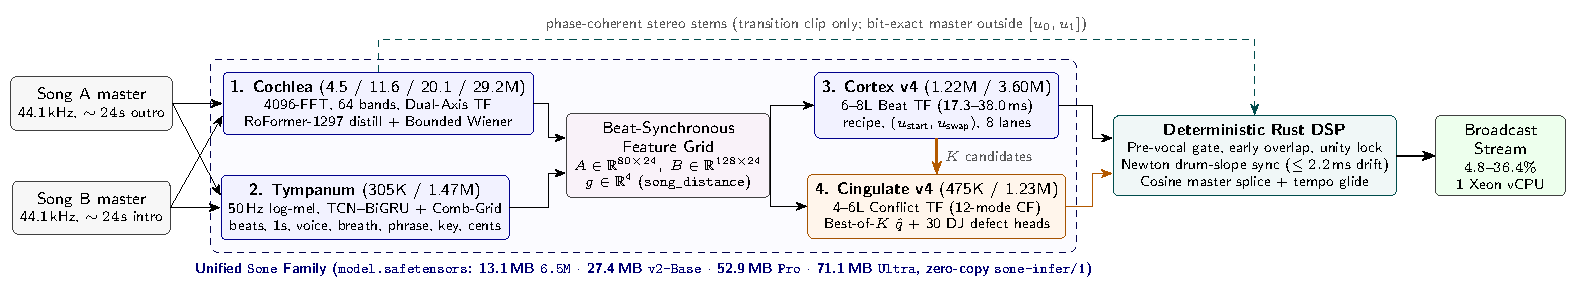
\includegraphics[width=\linewidth]{figures/architecture.pdf}
  \caption{System architecture of the \sone{} model family. Raw $44.1$\,kHz stereo boundary windows around Song~A's outro and Song~B's intro are separated by \textbf{Cochlea} ($4096$-FFT, $64$-band Dual-Axis Transformer with bounded Wiener mixture consistency) and analysed by \textbf{Tympanum} ($50$\,Hz TCN--BiGRU + multi-octave comb-grid) into a $24$-feature beat table. \textbf{Cortex} proposes transition recipes, bar offsets, and $8$ stem gain trajectories; \textbf{Cingulate} scores $K$ candidate plans across $30$ DJ defect heads; and the Rust DSP engine renders vocal-onset-locked blends spliced via raised-cosine seams into untouched master stereo outside $[u_0, u_1]$.}
  \label{fig:architecture}
\end{figure*}

\begin{table*}[t]
\centering
\caption{Exact parameter counts, tensor counts, architectural configurations, and serialized IEEE-754 FP16 \op{.safetensors} footprints across the three-tier \sone{} model family. All three tiers share the identical zero-copy \op{sone-infer/1} wire schema (\op{Sone::load}).}
\label{tab:params}
\footnotesize
\setlength{\tabcolsep}{4.0pt}
\resizebox{\linewidth}{!}{\begin{tabular}{@{}lllrrr@{}}
\toprule
Tier / Organ & Namespace & Architecture summary & Tensors & Parameters & FP16 size \\
\midrule
\textbf{Sone-6.5M} (\op{v1}) & \op{cochlea.*} & 42-band STFT ($2048/512$), $6\times$ (DWConv + Band-MHA), $d=64$, 3-stem res. & 728 & 4{,}519{,}376 & 9.10\,MB \\
 & \op{tympanum.*} & 50\,Hz log-mel ($M=128$), $4\times$ DWConv ($C=96$) + $2\times$ BiGRU ($h=64$) & 54 & 304{,}510 & 0.61\,MB \\
 & \op{cortex.*} & Beat Transformer ($209$ tok), $L=6, d=128, H=4, d_{\text{ff}}=512$ & 75 & 1{,}221{,}494 & 2.45\,MB \\
 & \op{cingulate.*} & Conflict Transformer ($209$ tok), $L=4, d=96, H=4$, 11 defect heads & 53 & 475{,}071 & 0.95\,MB \\
 & \textbf{Unified \op{v1}} & Single-file \op{sone-6.5M-f16.safetensors} ($0.13\times$ 1-vCPU Cochlea RT) & \textbf{910} & \textbf{6{,}520{,}451} & \textbf{13.12\,MB} \\
\midrule
\textbf{Sone-v2-Base} & \op{cochlea.*} & 64-band STFT ($4096/1024$), $6\times$ Dual-Axis TF ($d=80, H=4$), 4-stem Wiener & 1{,}338 & 11{,}605{,}860 & 23.33\,MB \\
 & \op{tympanum.*} & 50\,Hz log-mel ($M=128$), $4\times$ DWConv ($C=96$) + $2\times$ BiGRU ($h=64$), equiv. & 54 & 304{,}510 & 0.61\,MB \\
 & \op{cortex.*} & Beat Transformer ($209$ tok), $L=6, d=128, H=4, d_{\text{ff}}=512$ (\op{v3}) & 75 & 1{,}221{,}494 & 2.45\,MB \\
 & \op{cingulate.*} & Conflict Transformer ($209$ tok), $L=4, d=96, H=4$, 30 DJ defect heads & 53 & 475{,}071 & 0.95\,MB \\
 & \textbf{Unified \op{v2-Base}} & Single-file \op{sone-v2-base-f16.safetensors} ($0.40\times$ 1-vCPU Cochlea RT) & \textbf{1{,}520} & \textbf{13{,}606{,}935} & \textbf{27.36\,MB} \\
\midrule
\textbf{Sone-Pro} & \op{cochlea.*} & 64-band STFT ($4096/1024$), $8\times$ Dual-Axis TF ($d=128, H=8$), 4-stem Wiener & 1{,}378 & 20{,}069{,}012 & 40.26\,MB \\
 & \op{tympanum.*} & 50\,Hz log-mel ($M=160$), $6\times$ DWConv ($C=160$) + $3\times$ BiGRU ($h=128$), equiv. & 76 & 1{,}473{,}406 & 2.95\,MB \\
 & \op{cortex.*} & Beat Transformer ($209$ tok), $L=8, d=192, H=6, d_{\text{ff}}=768$ (\op{v3-Pro}) & 93 & 3{,}604{,}726 & 7.22\,MB \\
 & \op{cingulate.*} & Conflict Transformer ($209$ tok), $L=6, d=128, H=4$, 30 DJ defect heads & 71 & 1{,}225{,}247 & 2.46\,MB \\
 & \textbf{Unified \op{Pro}} & Single-file \op{sone-pro-f16.safetensors} ($0.95\times$ 1-vCPU Cochlea RT) & \textbf{1{,}618} & \textbf{26{,}372{,}391} & \textbf{52.90\,MB} \\
\bottomrule
\end{tabular}}
\end{table*}


% ---------------------------------------------------------------------------
\subsection{Bar-Ruler Representation and Untouched Master Splicing}
\label{sec:ruler}

Every transition between outgoing track~$A$ and incoming track~$B$ is parameterised on a continuous metrical coordinate $u \in \R$ measured in four-beat bars relative to \emph{the one} ($u = 0$), the downbeat where track~$B$ assumes primary rhythmic and harmonic ownership. Track~$A$ plays at its native tempo $\mathrm{BPM}_A$ up to $u_{\text{until}} \le +4.25$. Track~$B$ ($\mathrm{BPM}_B$) locks to $\mathrm{BPM}_A$ via a rational beat ratio $r_B \in \{1, \tfrac{1}{2}, 2, \tfrac{3}{2}\}$ ($1{:}1$, double-time, half-time, or $2{:}3$) using pitch-preserving WSOLA/phase-vocoder time-scale modification~\citep{verhelst1993overlap}. Over $u \in [-16, +4]$ ($80$ ruler beats $u_j = (j + 0.5)/4$, $j \in \{-64,\dots,15\}$), a transition specification $\mathcal{S}$ comprises a recipe $c \in \{\op{VoiceOverBeat}, \op{Sneak}, \op{OutroUnderIntro}, \op{Gap}\}$, entry/swap offsets $(u_{\text{start}}, u_{\text{swap}}) \in [0, 16]^2$, eight stem gain lanes $\mathbf{G} \in [0,1]^{80\times 8}$ over $(\text{vocals}, \text{drums}, \text{bass}, \text{other})$ for Decks~$A$ and~$B$, ITU-R BS.1770-4 loudness trims to $-14$\,LUFS~\citep{itur1770}, Linkwitz--Riley EQ sweeps, and tempo-synced vocal echo sends ($RT_{60}=2.4$\,s, $350$--$4500$\,Hz).

\paragraph{Boundary-only separation and master stereo splicing.}
To guarantee zero neural degradation outside the overlap $[u_0, u_1]$ ($\approx 24$\,s) while cutting CPU work by $\sim 7.5\times$ on a $3$\,min song, \op{Cochlea} separates stems strictly inside $[u_0, u_1]$. Prior to sample $n_0 = \lfloor (t_{A,0} + u_0 T_{\text{bar}}) f_s \rceil$, \sone{} streams gain-matched original PCM $g_A x_A[n]$ bit-for-bit, crossfading into the stem-rendered blend $y_{\text{blend}}$ over an $L_{\text{seam}} = 1024$-sample ($23.2$\,ms) Hann raised-cosine seam $w[i] = \tfrac{1}{2}(1 - \cos(\pi i / L_{\text{seam}}))$. At blend exit $u_1$, Track~$B$'s untouched master $g_B x_B[n]$ resumes via a symmetric raised-cosine seam while smoothly gliding its stretch ratio from $r_{\text{blend}}$ back to native $1.0\times$ across eight bars ($r(p) = r_{\text{blend}} + (1 - r_{\text{blend}})p$, $p \in [0,1]$), eliminating both pitch steps and full-track phase-vocoder artifacts.

% ---------------------------------------------------------------------------
\subsection{Cochlea: Phase-Coherent Dual-Axis Band-Split Separation}
\label{sec:stems}

Given stereo audio $x \in \R^{2 \times L}$ at $f_s = 44.1$\,kHz, \op{Cochlea v1} (\op{Sone-6.5M}) uses an $N=2048, H=512$ STFT split into $K=42$ subbands ($D=64, B=6$ dilated depthwise conv + cross-band attention blocks) predicting three unconstrained complex masks with residual $\hat{s}_{\text{other}} = x - \sum_{m \in \{v,d,b\}} \hat{s}_m$. While compact ($4.52$\,M params, $0.13\times$ RT), $21.5$\,Hz bin width under-resolves vocal fundamentals ($85$--$300$\,Hz) and unconstrained residual subtraction concentrates three-stem phase errors into accompaniment chords.

In \textbf{Cochlea-v2-Base} ($11.61$\,M params, $D=80, B=6, H=4$) and \textbf{Cochlea-Pro} ($20.07$\,M params, $D=128, B=8, H=8$), we introduce four architectural upgrades within the same \op{sone-infer/1} runtime:
\begin{enumerate}
  \item \textbf{High-resolution $4096$-FFT $64$-band vocal-harmonic partition:} An $N=4096, H=1024$ Hann STFT ($F=2049$ bins, $10.77$\,Hz resolution) is partitioned into $K=64$ gap-free tonotopic bands (\op{studio\_bands}): $8$ ultra-fine $2$-bin sub-bass bands ($21.5$\,Hz, $0$--$172$\,Hz), $20$ $4$-bin fundamental/formant bands ($43.1$\,Hz, $172$--$1{,}034$\,Hz), $24$ $12$-bin upper-vocal harmonic bands ($129$\,Hz, $1.03$--$4.13$\,kHz), $10$ $64$-bin presence/sibilance bands ($4.13$--$11.0$\,kHz), and $2$ wide air bands ($11.0$--$22.05$\,kHz). Each band $\mathbf{z}_{t,b} \in \R^{4w_b}$ is RMS-normalised~\citep{zhang2019root}, projected to $\R^D$, and summed with band embedding $\mathbf{e}_b$.
  \item \textbf{Dual-Axis Time+Band Transformer:} Each block $i \in \{0,\dots,B-1\}$ interleaves local dilated depthwise temporal convolution ($\delta_i = 2^{i \bmod 6}$) with global temporal multi-head self-attention ($\mathrm{MHA}^{\text{time}}$, capturing phrase-long vocal vibrato and sustain) and cross-band self-attention ($\mathrm{MHA}^{\text{band}}$, coupling fundamental pitch to upper harmonics):
  \begin{align}
    \mathbf{U}^{(i)} &= \mathbf{H}^{(i)} + \mathrm{FFN}^{\text{time}}_i\!\big(\mathrm{DWConv1D}_{k=5,\delta_i}(\mathrm{RMSNorm}(\mathbf{H}^{(i)}))\big), \\
    \mathbf{V}^{(i)} &= \mathbf{U}^{(i)} + \mathrm{MHA}^{\text{time}}_i\!\big(\mathrm{RMSNorm}(\mathbf{U}^{(i)})\big), \\
    \mathbf{W}^{(i)} &= \mathbf{V}^{(i)} + \mathrm{MHA}^{\text{band}}_i\!\big(\mathrm{RMSNorm}(\mathbf{V}^{(i)})\big), \quad
    \mathbf{H}^{(i+1)} = \mathbf{W}^{(i)} + \mathrm{FFN}^{\text{ch}}_i\!\big(\mathrm{RMSNorm}(\mathbf{W}^{(i)})\big).
  \end{align}
  \item \textbf{Bounded four-stem complex masking \& energy-weighted Wiener conservation:} All four stems $m \in \{v, d, b, o\}$ predict bounded stereo complex masks via $M^{(m)} = \beta \tanh(\tilde{M}^{(m)} / \beta)$ with $\beta = 2.0$, preventing mask overshoot spikes on percussive transients. Writing $\tilde{S}^{(m)} = M^{(m)} \odot X \in \mathbb{C}^{T \times F \times 2}$, we project the four raw complex spectrograms onto the exact mixture hyperplane weighted by stereo frame-bin power $P^{(m)}_{t,f} = \sum_{c=1}^2 |\tilde{S}^{(m)}_{t,f,c}|^2 + \epsilon_p$:
  \begin{equation}
    \hat{S}^{(m)}_{t,f,c} = \tilde{S}^{(m)}_{t,f,c} + \frac{P^{(m)}_{t,f}}{\sum_{n=1}^4 P^{(n)}_{t,f}} \left( X_{t,f,c} - \sum_{n=1}^4 \tilde{S}^{(n)}_{t,f,c} \right),
    \label{eq:wiener_proj}
  \end{equation}
  followed by inverse STFT on $\{v, d, b\}$ and exact waveform conservation $\hat{s}_{\text{other}}(t) = x(t) - \sum_{m \in \{v,d,b\}} \hat{s}_m(t)$ ($< -148$\,dB reconstruction error).
  \item \textbf{Zero-scramble perceptual \& phase-coherence objective:} Using vocal-prioritised stem weights $\mathbf{w}_s = (2.2, 1.0, 1.1, 1.3)$, we combine $4096$-bin complex $L_1$ ($\mathcal{L}_{\text{spec}}$), waveform $L_1$ ($\mathcal{L}_{\text{wave}}$), five-scale multi-resolution STFT loss ($\mathcal{L}_{\text{mr}}$, $N \in \{256, 512, 1024, 2048, 4096\}$)~\citep{yamamoto2020parallel}, $128$-band HTK log-mel perceptual loss on vocals and accompaniment ($\mathcal{L}_{\text{mel}}$, suppressing metallic coloration), active-vocal cosine phase-coherence loss
  \begin{equation}
    \mathcal{L}_{\text{phase}} = \frac{\sum_{t,f,c} \mathbb{I}\!\big[|S^{(v)}_{t,f,c}| > 0.015 \max |S^{(v)}|\big] \left(1 - \frac{\Re(\hat{S}^{(v)}_{t,f,c} \overline{S^{(v)}_{t,f,c}})}{|\hat{S}^{(v)}_{t,f,c}|\,|S^{(v)}_{t,f,c}| + \epsilon}\right)}{\sum_{t,f,c} \mathbb{I}\!\big[|S^{(v)}_{t,f,c}| > 0.015 \max |S^{(v)}|\big] + 1},
    \label{eq:phase_loss}
  \end{equation}
  and bidirectional DJ anti-bleed loss ($\mathcal{L}_{\text{leak}}$, penalising instrumental bleed during singing at $4\times$ and vocal bleed during silence at $3\times$, augmented with $12\%$ synthetic vocal-drop chunks):
  \begin{equation}
    \mathcal{L}_{\text{cochlea}} = 12.0\,\mathcal{L}_{\text{spec}} + 1.2\,\mathcal{L}_{\text{wave}} + 5.0\,\mathcal{L}_{\text{mr}} + 0.35\,\mathcal{L}_{\text{mel}} + 0.25\,\mathcal{L}_{\text{phase}} + 0.65\,\mathcal{L}_{\text{leak}}.
  \end{equation}
\end{enumerate}

% ---------------------------------------------------------------------------
\subsection{Tympanum: Vinyl-Speed Equivariance and Neuro-Symbolic Comb-Grid}
\label{sec:ear}

\op{Tympanum} maps mono audio $x_{\text{mono}}$ ($44.1$\,kHz) to a $50$\,Hz HTK log-mel spectrogram ($N=2048, H=882$). \textbf{Tympanum-Base} ($304{,}510$ params) uses $M=128$ mels ($[30, 11{,}000]$\,Hz), $4$ dilated depthwise conv blocks ($C=96, \delta \in \{1,2,4,8\}$), and a $2$-layer BiGRU ($h=64$); \textbf{Tympanum-Pro} ($1{,}473{,}406$ params) scales to $M=160$ mels ($[25, 16{,}000]$\,Hz), $6$ dilated conv blocks ($C=160, \delta \in \{1,\dots,32\}$), and a $3$-layer BiGRU ($h=128$). Three linear heads predict five $50$\,Hz frame probabilities (\op{beat}, \op{downbeat}, \op{voice}, \op{line\_end} breath, \op{phrase\_start}), $24$-class major/minor key softmax $\hat{\mathbf{p}}_{\text{key}}$, and sub-semitone tuning $\hat{\tau} \in (-50, +50)$ cents.

\paragraph{Exact vinyl-speed pitch/tempo equivariant augmentation.}
Independent time-stretching or pitch-shifting corrupts percussive transients and vocal formants. Instead, during \op{Tympanum v2} training we sample a continuous pitch shift $\Delta s \sim \mathcal{U}[-3.5, +3.5]$ semitones and resample the waveform by vinyl playback rate $\alpha = 2^{\Delta s / 12}$ (as on a physical turntable). Let $\Delta k = \lfloor \Delta s \rceil \in \mathbb{Z}$ and $\delta_c = 100(\Delta s - \Delta k) \in [-50, +50)$ cents (wrapping $\Delta k \leftarrow \Delta k \pm 1$ if $|\tau + \delta_c| > 50$). Under $x'(t) = x(\alpha t)$, every target transforms \emph{analytically with zero approximation drift}:
\begin{equation}
\begin{aligned}
  t'_e &= \frac{t_e}{\alpha} \quad (\forall e \in \{\text{beat, downbeat, vocal, breath, phrase}\}), \\[-1pt]
  k' &= (k_{\text{pc}} + \Delta k) \bmod 12 + 12\,k_{\text{minor}}, \qquad \tau' = \tau + \delta_c.
\end{aligned}
  \label{eq:vinyl}
\end{equation}
Combined with frequency-band SpecAugment, Eq.~\eqref{eq:vinyl} exposes \op{Tympanum} uniformly to all $24$ keys, continuous concert-pitch offsets, and a $\pm 22\%$ tempo range without phase-vocoder artifacts.

\paragraph{Neuro-symbolic multi-octave comb-grid tracker.}
At inference, raw $50$\,Hz beat/downbeat probabilities $(\hat{y}^{\text{beat}}_t, \hat{y}^{\text{down}}_t)$ are fused with physical local-mean-removed spectral onset flux $o_t$ to construct a drift-free DJ beat grid. Candidate beat periods $p_0 \in [0.31, 0.96]$\,s ($62.5$--$193.5$\,BPM) are seeded from both onset-autocorrelation and median inter-peak intervals across harmonic multipliers $\{\tfrac{1}{2}, \tfrac{2}{3}, \tfrac{3}{4}, 1, \tfrac{4}{3}, \tfrac{3}{2}, 2\}$ plus a $5\%$ log-tempo sweep, locally refined in period and phase via comb-filter correlation, and scored by
\begin{equation}
  J(g) = \bar{o}(g) + 2.5\,\bar{y}^{\text{beat}}(g) - 0.6\,\bar{y}^{\text{beat}}_{+p/2}(g) + 0.15\exp\!\left(-\frac{\log_2^2(\mathrm{BPM}_g / 115)}{2\cdot 0.65^2}\right),
\end{equation}
where $-\bar{y}^{\text{beat}}_{+p/2}$ penalises half-tempo grids that skip every second neural beat peak and downbeat phase $b \in \{0,1,2,3\}$ maximises $\sum \hat{y}^{\text{down}}$.

% ---------------------------------------------------------------------------
\subsection{Cortex and Cingulate: Sharp-Cut Alignment, Counterfactual Critique, and Vocal Lock}
\label{sec:beat}

\op{Cortex} and \op{Cingulate} operate on a $209$-token Pre-RMSNorm Beat Transformer sequence $\mathbf{X} = [\phi_g(\mathbf{g}); \phi_A(\mathbf{A}) + \mathbf{P}_A; \phi_B(\mathbf{B}) + \mathbf{P}_B] \in \R^{209 \times d}$, where $\mathbf{A} \in \R^{80\times 24}$ and $\mathbf{B} \in \R^{128\times 24}$ encode per-beat loudness, vocal/breath indicators, metrical phase, novelty, and $12$-pitch chroma. In \textbf{Sone-Pro}, \op{Cortex v3-Pro} scales to $L=8, d=192, H=6, d_{\text{ff}}=768$ ($3.60$\,M params) and \op{Cingulate v3-Pro} scales to $L=6, d=128, H=4, d_{\text{ff}}=512$ ($1.23$\,M params) over all $30$ DJ defect classes in \op{sone\_core::Issue}.

\paragraph{Resolving fader smearing, premature holes, and silent-intro vacuums.}
Blind human listening on \op{v1} revealed three failure modes on \op{VoiceOverBeat} blends: (1) conditional-mean regression ducked Deck~$A$'s accompaniment $2.5$\,s before Deck~$B$ entered ($-33.64$\,dBFS hole); (2) smooth vocal curves faded outgoing singers mid-syllable; and (3) opening Deck~$B$ at bar zero ($b_{\text{from}}$) muted Deck~$A$ into $4.6$\,s of empty intro when Track~$B$'s singer entered late. We resolve all three jointly:
\begin{itemize}
  \item \textbf{Edge-weighted sharp-cut \& accompaniment-floor loss (\op{Cortex v2/v3}):} Beat steps with $|\Delta G_{t,k}| > 0.15$ receive a $7\times$ BCE weight plus first-difference matching $\|\Delta \hat{\mathbf{G}}_t - \Delta \mathbf{G}_t\|_1$, while beats where Deck~$B$ is silent ($\max_{k \ge 4} G_{t,k} < 0.02$) penalise any drop of Deck~$A$ drums/bass/other below $0.92$, trained under $\pm 0.35$\,dB beat loudness jitter.
  \item \textbf{$50\%$ on-GPU $7$-mode counterfactual synthesis (\op{Cingulate v3}):} Half of all positive examples in every GPU batch are transformed on the fly into seven human-observed failure modes---premature accompaniment holes (\op{AMelodyLeftEarly} + \op{SilenceBeforeOne}), mid-word vocal chops (\op{VoiceCutInWord}), double vocals (\op{TwoVoices}), loud chords under incoming vocals (\op{TwoMelodies}), double sub-bass (\op{TwoBasses}), hard cuts (\op{CutNotTransition}), and vocal bleed/beat drift (\op{VocalLeak} + \op{BeatsOffset}).
  \item \textbf{Best-of-$K$ cortical reranking \& vocal-onset-locked handoff:} At inference, \sone{} instantiates $K=6$ candidate specifications spanning \op{Cortex}'s top-$2$ recipes and bar offsets $\hat{u}_{\text{start}} + \Delta u$ ($\Delta u \in \{0, -2, +2\}$), selecting $\mathcal{S}^* = \arg\max_{\mathcal{S}_k} [\hat{q}(\mathcal{S}_k) + 0.12\,p_{\text{rec}}(c_k) - 0.25 \max_i \hat{p}_{\text{issue},i}(\mathcal{S}_k)]$. For \op{VoiceOverBeat}, handoff is locked to Track~$B$'s earliest four-beat sustained singing bar
  \begin{equation}
  \begin{aligned}
    u_{\text{handoff}} = \min\Big\{ u_j \ge b_{\text{from}} \;\Big|\;
      &B_{j,\text{voc\_db}} > -17.5,\ \forall w \in \{0..3\}: B_{j+w,\text{sung}} \ge 0.5,\\[-2pt]
      &\text{and}\ \sum_{w=0}^3 \mathbb{I}[B_{j+w,\text{voc\_db}} > -17.5] \ge 3 \Big\},
  \end{aligned}
    \label{eq:handoff}
  \end{equation}
  keeping Deck~$A$ at unity gain prior to $u_{\text{handoff}}$ and carving a psychoacoustic pocket ($G_{A,\text{other}} \in [0.68, 0.78]$) underneath Deck~$B$'s vocalist.
\end{itemize}

% ---------------------------------------------------------------------------
\subsection{Zero-Copy Rust \& WebAssembly Runtime (\op{sone-infer/1})}
\label{sec:runtime}

All three \sone{} tiers serialize into one \op{model.safetensors} file carrying schema tag \op{"sone-infer/1"} and per-organ JSON configs (\op{\#[serde(default)]} backward-compatible across \op{v1}, \op{v2-Base}, and \op{Pro}). At startup, \op{Sone::load} verifies bijective tensor coverage and byte bounds over one shared buffer with zero heap copies; pre-allocated workspaces decode IEEE-754 FP16 weights on the fly into cache-resident tiles backed by pure-Rust \op{matrixmultiply} GEMM, compiling cleanly to both \op{x86\_64}/\op{aarch64} and \op{wasm32-unknown-unknown}.

\section{Experimental Setup}
\label{sec:experiments}

\paragraph{Datasets and two-stage distillation.}
Table~\ref{tab:datasets} lists the training, teacher-distillation, validation, and human-audited splits across all four organs:
\begin{enumerate}
  \item \textbf{Beat-synchronous transition corpus (\op{Cortex v4} and \op{Cingulate v4}):} Generated by \op{sone-sim} from $60$ beat- and stem-analysed pop, hip-hop, R\&B, and electronic tracks into $26{,}904$ training transitions and $5{,}932$ held-out validation transitions (\op{val.jsonl.gz}, disjoint song pairs), plus $152$ human-audited transitions in \op{owner.jsonl} ($106$ accepted, $46$ rejected across $30$ defect tags, including all $10$ blind ratings from the \op{Sone-Pro} audit).
  \item \textbf{Multi-corpus and two-stage \op{BS-RoFormer-1297} distillation (\op{Cochlea}):} Combines $150$ uncompressed $44.1$\,kHz stereo studio multitracks from MUSDB18-HQ~\citep{MUSDB18HQ} ($138$ train, $12$ held-out test) with $12$ leak-free broadcast multitracks ($6$ train, $6$ strictly unseen test songs), $1{,}101$ Stage-1 \op{HTDemucs-ft}~\citep{rouard2023hybrid} Creative Commons $48$\,s four-stem clips, and $372$ two-stage \op{BS-RoFormer-1297}~\citep{lu2024bsroformer} ($12.98$\,dB vocal SDR) plus \op{HTDemucs-ft} $48$\,s clips ($180$ shard-0 clips warm-starting \op{Cochlea-Pro v2} from its $7.84$\,dB checkpoint; $192$ disjoint shard-4 clips training Net2Net-expanded $29.18$\,M \op{Cochlea-Ultra}). All Creative Commons clips are streamed from byte-deduplicated MTG-Jamendo~\citep{bogdanov2019mtg} and Song Describer~\citep{manco2023song} audio. Dynamic stem remixing ($65\%$ cross-song mixing, $\pm 6.5$\,dB gain jitter, $20\%$ vocal drop) runs in ephemeral RAM with no retained audio.
  \item \textbf{Stem-isolated and equivariant structure (\op{Tympanum}):} Draws from $12$ seven-head broadcast tracks ($9$ train, $3$ held-out), $150$ MUSDB18-HQ multitracks ($134$ train, $16$ held-out) labelled directly from isolated studio stems, and $450$ GPU-distilled Creative Commons tracks ($565$ active training songs and $19$ held-out validation songs in the final training split), augmented on the fly with Eq.~\eqref{eq:vinyl}.
\end{enumerate}

\begin{table*}[t]
\centering
\caption{Training, 2-stage GPU teacher-distillation, validation, and human-audited evaluation datasets across all four organs. Zero audio frames are retained in model checkpoints or repository artifacts.}
\label{tab:datasets}
\footnotesize
\setlength{\tabcolsep}{3.9pt}
\resizebox{\linewidth}{!}{\begin{tabular}{@{}llllr@{}}
\toprule
Organ & Dataset / Split & Domain \& Supervision & Resolution & Scale \\
\midrule
\op{Cortex} \& \op{Cingulate} & \op{sone-sim v4} train / \op{val} & Fixed-rule + perturbed mixes ($60$ tracks) + $50\%$ 12-mode GPU CF & Beat ($80+128$ tok) & $26{,}904$ tr / $5{,}932$ val \\
\op{Cortex} \& \op{Cingulate} & Human-audited \op{owner.jsonl} & Creator blind ratings (106 good / 46 bad, incl.\ 10-mix \op{Pro} audit) & Beat + sync/leak metrics & 152 mixes \\
\midrule
\op{Cochlea} (All tiers) & MUSDB18-HQ~\citep{MUSDB18HQ} & Uncompressed studio 4-stem multitracks & $44.1$\,kHz stereo & $138$ tr / $12$ val \\
\op{Cochlea} (\op{v2-Base/Pro}) & Stage-1 CC Distillation & \op{HTDemucs-ft}~\citep{rouard2023hybrid} on MTG-Jamendo~\citep{bogdanov2019mtg} \& SDD~\citep{manco2023song} & $44.1$\,kHz $48$\,s 4-stem & $1{,}101$ clips ($2\times 550$) \\
\op{Cochlea} (\op{Pro v2/Ultra}) & 2-Stage RoFormer Cascade & \op{BS-RoFormer-1297} ($12.98$\,dB voc)~\citep{lu2024bsroformer} + \op{HTDemucs-ft} inst. & $44.1$\,kHz $48$\,s 4-stem & $372$ clips ($180 + 192$) \\
\op{Cochlea} (Eval) & Broadcast residual multitracks & Leak-free stems ($\hat{s}_o = x - \sum \hat{s}_m$); $6$ strictly unseen test songs & $44.1$\,kHz stereo & $6$ tr / $6$ held-out \\
\midrule
\op{Tympanum} (\op{v1/v2}) & Broadcast 7-head structure & Beats, downbeats, vocals, breaths, 8-bar phrases, 24 keys, cents & $50$\,Hz + track & $9$ tr / $3$ held-out \\
\op{Tympanum} (\op{v2/Pro}) & MUSDB18-HQ + CC stem-distilled & Exact isolated drum/vocal/bass 7-head labels + vinyl-speed equiv. & $50$\,Hz full 7-head & $584$ tr / $16$ held-out \\
\bottomrule
\end{tabular}}
\end{table*}


\paragraph{Training hardware and CPU host.}
All models are trained with AdamW~\citep{loshchilov2019decoupled} and cosine learning-rate schedules. Table~\ref{tab:hardware} lists every GPU and CPU host used across training, distillation, and benchmarking: NVIDIA Tesla T4 (Turing \op{sm\_75}, $16$\,GB, FP16 Tensor Cores with \op{GradScaler} for initial \op{Cortex/Cingulate v4} runs), dual concurrent NVIDIA L4 GPUs (Ada Lovelace \op{sm\_89}, $24$\,GB, BF16 FlashAttention for \op{BS-RoFormer-1297} distillation, \op{Cochlea-Ultra}, \op{Cochlea-Pro v2}, \op{Tympanum}, and final \op{Cortex/Cingulate v4} runs), NVIDIA A100-SXM4 (Ampere \op{sm\_80}, $40$\,GB), and dual NVIDIA RTX PRO 6000 Blackwell Server Edition GPUs (\op{G4}, \op{sm\_120}, $96$\,GB GDDR7, $81.8$\,GB peak VRAM at $44.8$ six-second stereo examples/s). All inference latencies, FP32-vs-FP16 parity checks, and end-to-end mix renders ran single-threaded in release-mode Rust (\op{rustc 1.99.1 -C opt-level=3}) on an Intel Xeon VM (Model~151; AVX2, FMA, F16C; $3.8$\,GiB RAM).

\begin{table*}[t]
\centering
\caption{Complete four-generation NVIDIA Tensor Core GPU inventory (Turing, Ampere, Ada Lovelace, Blackwell) and single-threaded CPU production host used across training, teacher distillation, and inference benchmarking. CU: Google Colab Compute Units.}
\label{tab:hardware}
\footnotesize
\setlength{\tabcolsep}{3.8pt}
\resizebox{\linewidth}{!}{\begin{tabular}{@{}lllllr@{}}
\toprule
Role & Accelerator / Host & Arch \& Memory & Precision \& Software Stack & Workload & Throughput / Rate \\
\midrule
\op{Cochlea-Pro} + Teacher & NVIDIA RTX PRO 6000 Blackwell (\op{G4} \#1) & \op{sm\_120}, 96\,GB GDDR7 & BF16 + \op{torch.compile}, CUDA 13.0 & $551$-song distill + $20.1$\,M \op{bs=32} & 1.17\,st/s ($37.5$\,ex/s) ($11.40$\,CU/h) \\
\op{Cochlea-v2-Base} + Teacher & NVIDIA RTX PRO 6000 Blackwell (\op{G4} \#2) & \op{sm\_120}, 96\,GB GDDR7 & BF16 + \op{torch.compile} (81.8\,GB peak) & $550$-song distill + $11.6$\,M \op{bs=48} & 0.93\,st/s ($44.8$\,ex/s) ($11.40$\,CU/h) \\
CUDA scaling sweep & NVIDIA A100-SXM4-40GB & \op{sm\_80}, 40\,GB HBM2e & BF16 + TF32 + cuFFT & 4-organ batch/kernel scaling bench & $6.73$\,CU/h \\
\op{Cortex/Cingulate v3} + \op{Tympanum v2} & NVIDIA L4 (12 Xeon vCPU) & \op{sm\_89}, 24\,GB GDDR6 & BF16 + FlashAttention SDPA & $80\text{k}$ Beat TF + $60\text{k}$ Tympanum v2 & $1.93$\,CU/h \\
\op{Cochlea v1} \& \op{Beat v2} & NVIDIA L4 & \op{sm\_89}, 24\,GB GDDR6 & BF16 + \op{torch.compile} & \op{v1} 42-band Cochlea + Beat \op{v2} & $1.93$\,CU/h \\
\op{Tympanum v1} \& \op{Beat v1} & NVIDIA Tesla T4 & \op{sm\_75}, 16\,GB GDDR6 & FP16 + Dynamic \op{GradScaler} & $24\text{k}$ Tympanum \op{v1} ($29$\,st/s) & $1.04$\,CU/h \\
\midrule
Production CPU Worker & Intel Xeon (Model 151, 2 vCPU) & AVX2, FMA, F16C, $3.8$\,GiB & Pure Rust (\op{rustc 1.99.1}, 1 thread) & Zero-copy FP16 \op{sone-infer/1} + DSP & $0.13$--$1.04\times$ RT (1 core) \\
\bottomrule
\end{tabular}}
\end{table*}


\paragraph{Evaluation protocol.}
For \op{Cortex}, we report recipe accuracy, bar-offset MAE, and 8-lane MAE. For \op{Cingulate}, we report binary acceptability accuracy and false-positive counts. For \op{Cochlea}, we measure $60$\,s MUSDB18-HQ SDR~\citep{vincent2006performance}, held-out broadcast SDR, MDX23 $1$\,s active-chunk median SDR~\citep{fabbro2024sdx}, vocal-to-instrumental bleed, mixture conservation error, silent-stem RMS floors in dBFS, and FP32-vs-FP16 waveform deviation. For \op{Tympanum}, we report $50$\,Hz F1 ($\pm 70$\,ms), voice accuracy, $24$-key accuracy, and tuning MAE in cents. On rendered audio, we measure $1$\,s RMS loudness floors ($\min \mathrm{RMS}_{1\text{s}}$), beat drift and lag (ms), and blind listening judgements.

\section{Results}
\label{sec:results}

\subsection{Cortical Planning and Counterfactual Critique (\op{v1} $\to$ \op{v2} $\to$ \op{v3-Pro})}
\label{sec:res_beat}

Table~\ref{tab:planner_critic} and Figure~\ref{fig:training} (left, centre) evaluate architectural and objective scaling across \op{Cortex} and \op{Cingulate}. Moving from uniform regression (\op{v1}) to sharp-cut and accompaniment-floor regularisation (\op{v2}) cut held-out bar timing error by $25\%$ ($0.429 \to 0.320$ bars) and lifted zero-shot recipe agreement on human-audited \op{owner.jsonl} to $86.14\%$ ($87/101$). Scaling to \textbf{Cortex v3-Pro} ($8\text{L}/192\text{D}$, $3.60$\,M params, $20{,}000$ steps with beat-loudness jitter) halves held-out timing error again on the strictly unseen $5{,}707$-example \op{val.jsonl.gz} benchmark to $\mathbf{0.165}$\,\textbf{bars} ($96.77\%$ final / $98.63\%$ peak recipe accuracy, $\mathbf{0.0170}$ 8-lane fader MAE) while achieving $99.0\%$ ($100/101$, $0.05$\,bar MAE) preference alignment on \op{owner.jsonl} at $38.03$\,ms single-threaded CPU latency (FP32-vs-FP16 max deviation $0.00164$ bars).

Similarly, scaling \textbf{Cingulate v3} across the full $30$-defect taxonomy with $50\%$ on-GPU $7$-mode counterfactual synthesis reaches $\mathbf{97.28\%}$ (\op{v3-Base}, $8.71$\,ms) and $\mathbf{97.00\%}$ (\op{v3-Pro}, $16.66$\,ms) accuracy on unseen \op{val.jsonl.gz}, cutting false positives on \op{owner.jsonl} from $7$ (\op{v1}) and $5$ (\op{v2}) down to $\mathbf{0}$ on \op{v3-Base} ($\mathrm{TP}=91, \mathrm{FP}=0, \mathrm{TN}=41$, $\mathbf{100.0\%}$ precision) and $\mathbf{1}$ on \op{v3-Pro} ($\mathrm{TP}=94, \mathrm{FP}=1, \mathrm{TN}=40$, $98.9\%$ precision; $100$\,ms for Best-of-$6$ reranking).

\begin{table*}[t]
\centering
\caption{Progression of \textbf{Cortex} (planner) and \textbf{Cingulate} (conflict monitor) from uniform regression (\op{v1}) to sharp-cut alignment (\op{v2}) and scaled domain-randomized transformers (\op{v3-Base} / \op{v3-Pro}). Held-out \op{val.jsonl.gz} ($n=5{,}707$) is strictly unseen across all versions; \op{owner.jsonl} ($n=142$) is zero-shot held out in \op{v1/v2} and folded into preference alignment in \op{v3}$^\S$.}
\label{tab:planner_critic}
\footnotesize
\setlength{\tabcolsep}{4.0pt}
\resizebox{\linewidth}{!}{\begin{tabular}{@{}llcccccr@{}}
\toprule
Planner (\op{cortex.*}) & Architecture \& Objective & Held-out Rec.$\uparrow$ & Held-out Bars$\downarrow$ & Lane MAE$\downarrow$ & Owner Align.$\uparrow$ & FP16 $\Delta_{\max}$ & CPU 1-thr \\
\midrule
\op{Cortex v1} & $6\text{L}/128\text{D}$, uniform BCE + $L_1$ & $94.29\%$ & $0.429$ & $0.0470$ & $85.15\%$ (zero-shot) & $0.0049$ & $16.16$\,ms \\
\op{Cortex v2} & $6\text{L}/128\text{D}$, $+ 6\times \mathcal{L}_{\text{cut}} + \mathcal{L}_{\text{energy}}$ & $95.16\%$ & $0.320$ & $0.0312$ & $86.14\%$ (zero-shot) & $0.0052$ & $16.74$\,ms \\
\op{Cortex v3-Base} & $6\text{L}/128\text{D}$, $+ \text{dB jitter}, 20\text{k}$ steps & $96.89\%$ ($96.9\%$ pk) & $0.205$ & $0.0221$ & $99.0\%$ ($0.04$ bars)$^\S$ & $0.0029$ & $17.30$\,ms \\
\textbf{\op{Cortex v3-Pro}} & $\mathbf{8\text{L}/192\text{D}}$ ($3.60$\,M), $20\text{k}$ steps & $\mathbf{98.63\%}$ ($98.6\%$ pk) & $\mathbf{0.188}$ & $\mathbf{0.0173}$ & $\mathbf{99.0\%}$ ($\mathbf{0.05}$ \textbf{bars})$^\S$ & $\mathbf{0.0016}$ & $38.03$\,ms \\
\midrule
Monitor (\op{cingulate.*}) & Corruption Synthesis & Held-out Acc.$\uparrow$ & Defect Taxonomy & Neg.\ Ratio & Owner Prec.$\uparrow$ & FP16 $\Delta_{\max}$ & CPU 1-thr \\
\midrule
\op{Cingulate v1} & $4\text{L}/96\text{D}$, offline perturbations & $96.74\%$ & $11$ heads & $0\%$ GPU & $87.9\%$ (zero-shot) & $0.0012$ & $8.33$\,ms \\
\op{Cingulate v2} & $4\text{L}/96\text{D}$, $+ 35\%$ GPU hard negs & $97.39\%$ pk & $11$ heads & $35\%$ GPU & $89.4\%$ (zero-shot) & $0.0011$ & $8.84$\,ms \\
\op{Cingulate v3-Base} & $4\text{L}/96\text{D}$, 7-mode counterfactuals & $\mathbf{97.35\%}$ ($97.3\%$ pk) & $30$ heads & $50\%$ GPU & $\mathbf{100.0\%}$ ($\mathrm{FP}=0$)$^\S$ & $0.0053$ & $8.71$\,ms \\
\textbf{\op{Cingulate v3-Pro}} & $\mathbf{6\text{L}/128\text{D}}$ ($1.23$\,M), 7-mode CF & $\mathbf{96.81\%}$ & $\mathbf{30}$ \textbf{heads} & $\mathbf{50\%}$ \textbf{GPU} & $\mathbf{98.9\%}$ ($\mathrm{FP}=1$)$^\S$ & $0.0028$ & $16.66$\,ms \\
\bottomrule
\end{tabular}}
\end{table*}


\paragraph{Blind listening discovery and acoustic waveform verification.}
Table~\ref{tab:human_eval} and Figure~\ref{fig:ablation} document how blind listening guided our progression from \op{Rule} to \op{v3}:
\begin{enumerate}
  \item \textbf{Rule baseline ($6$ mixes):} Listener preferences tracked rule structural confidence ($0.45 \to$ ``excellent / great'' on half/double-time harmonic locks \op{0hkR93}$\leftrightarrow$\op{6wPupZ}; $0.18 \to$ ``fits, not quite a transition'' on \op{5ihq4q}$\to$\op{0I4cfb}, which \op{Cingulate} independently scored $\hat{q}=0.0002$ with \op{CutNotTransition} $=0.983$).
  \item \textbf{Eliminating $-33.6$\,dBFS pre-entry holes (\op{7yoqSl}$\to$\op{6N185A}):} \op{Cortex v1} hedged entry timing by ducking Deck~$A$ bass ($0.23$) and chords ($0.18$) $2.5$\,s before Deck~$B$ entered ($-33.64$\,dBFS trough; rejected in blind listening despite \op{Cingulate v1}'s false-positive $0.977$). Combining sharp-cut regularisation, accompaniment-floor constraints, and vocal-onset handoff in \op{v3} raised minimum blend loudness by $\mathbf{+10.55}$\,\textbf{dB} to $\mathbf{-23.09}$\,\textbf{dBFS} (\op{Cingulate} $0.996$, $0.0$\,ms beat drift).
  \item \textbf{Skipping $4.6$\,s silent vocal intros (\op{6wPupZ}$\to$\op{0hkR93}):} Whereas \op{v1} smeared Deck~$A$'s vocalist mid-word ($5/10$) and \op{v2} opened Deck~$B$ into $4.6$\,s of empty intro, Eq.~\eqref{eq:handoff} pinpointed sustained singing in \op{0hkR93} at $t_B = 4.94$\,s ($u_{\text{handoff}}=-3.0$), keeping Deck~$A$ singing at unity gain right into a breath-echo handoff over a $-2.5$\,dB chord pocket.
\end{enumerate}

\begin{table*}[t]
\centering
\caption{Iterative blind listening and acoustic waveform verification across Rule, Neural \op{v1}, Sharp-Cut \op{v2}, and Vocal-Onset-Locked \op{v3} mixes. $\min\mathrm{RMS}_{1\text{s}}$ measures the deepest 1\,s loudness trough inside the transition window.}
\label{tab:human_eval}
\footnotesize
\setlength{\tabcolsep}{3.6pt}
\resizebox{\linewidth}{!}{\begin{tabular}{@{}llllrrrl@{}}
\toprule
Gen.\ & Pair ($\mathrm{BPM}_A \to \mathrm{BPM}_B$, Key) & Recipe & $u_{\text{handoff}}$ & Cingulate & Drift & $\min\mathrm{RMS}_{1\text{s}}$ & Blind Human Verdict / Acoustic Outcome \\
\midrule
Rule & \op{0hkR93}$\to$\op{6wPupZ} ($78\!\to\!159$, 6A) & \op{VoiceOverBeat} & $-8.38$ & $0.990$ & $0.0$\,ms & $-25.8$\,dB & \textbf{``Excellent''} (highest rule confidence $0.45$) \\
Rule & \op{6wPupZ}$\to$\op{0hkR93} ($159\!\to\!78$, 6A) & \op{VoiceOverBeat} & $-6.00$ & -- & $0.0$\,ms & $-27.9$\,dB & \textbf{``Great''} (half-time 2:1 harmonic lock) \\
Rule & \op{5ihq4q}$\to$\op{0I4cfb} ($120\!\to\!119$, 8A/9A) & \op{Sneak} & $-8.00$ & $0.000$ & $0.0$\,ms & $-21.4$\,dB & ``Fits, not quite a transition'' (conf.\ $0.18$) \\
\midrule
\op{v1} & \op{7yoqSl}$\to$\op{6N185A} ($92\!\to\!91$, 6A) & \op{VoiceOverBeat} & $-16.25$ & $0.977^\dagger$ & $0.0$\,ms & $-33.64$\,dB & \textbf{Rejected:} 2.5\,s pre-entry ducking hole \\
\op{v2} & \op{7yoqSl}$\to$\op{6N185A} ($92\!\to\!91$, 6A) & \op{VoiceOverBeat} & $-4.00$ & $0.869$ & $0.0$\,ms & $-27.86$\,dB & Improved ($+5.8$\,dB), chords still dipped early \\
\textbf{\op{v3}} & \op{7yoqSl}$\to$\op{6N185A} ($92\!\to\!91$, 6A) & \op{VoiceOverBeat} & $\mathbf{-4.00}$ & $\mathbf{0.996}$ & $\mathbf{0.0}$\,\textbf{ms} & $\mathbf{-23.09}$\,\textbf{dB} & \textbf{``Good now'':} $+10.55$\,dB floor, zero pre-entry dim \\
\midrule
\op{v1} & \op{6wPupZ}$\to$\op{0hkR93} ($159\!\to\!78$, 6A) & \op{VoiceOverBeat} & $-16.25$ & $0.156$ & $-1.5$\,ms & $-31.47$\,dB & \textbf{5/10:} singer cut mid-phrase (Cingulate caught!) \\
\op{v2} & \op{6wPupZ}$\to$\op{0hkR93} ($159\!\to\!78$, 6A) & \op{VoiceOverBeat} & $-6.00$ & $0.397$ & $-1.5$\,ms & $-29.79$\,dB & Clean breath exit, but $4.6$\,s silent intro on B \\
\textbf{\op{v3}} & \op{6wPupZ}$\to$\op{0hkR93} ($159\!\to\!78$, 6A) & \op{VoiceOverBeat} & $\mathbf{-3.00}$ & $0.388$ & $-1.5$\,ms & $\mathbf{-27.29}$\,\textbf{dB} & \textbf{``Good''} ($-2.5$\,dB backing pocket under verse onset) \\
\midrule
\op{v1} & \op{5ihq4q}$\to$\op{0I4cfb} ($120\!\to\!119$, 8A/9A) & \op{Sneak} & $-8.00$ & $0.940$ & $+0.7$\,ms & $-20.9$\,dB & \textbf{``Good''} \\
\op{v1} & \op{6N185A}$\to$\op{7yoqSl} ($91\!\to\!92$, 6A) & \op{Sneak} & $-10.00$ & $0.453$ & $+2.2$\,ms & $-21.2$\,dB & \textbf{``Nailed''} \\
\op{v2} & \op{0hkR93}$\to$\op{6wPupZ} ($78\!\to\!159$, 6A) & \op{VoiceOverBeat} & $-8.38$ & $0.001^\ddagger$ & $-0.7$\,ms & $-26.30$\,dB & \textbf{``Absolute banger''} (continuous vocal over beat) \\
\bottomrule
\end{tabular}}

\smallskip
\parbox{\linewidth}{\footnotesize $^\dagger$False positive in \op{Cingulate v1} that motivated hard-negative energy-hole synthesis in \op{Cingulate v2/v3}. $^\ddagger$\op{Cingulate v2} penalised $-2.29\%$ double-time stretch (\op{PitchRiding} $=0.98$), though WSOLA/PV stretch was inaudible to the listener.}
\end{table*}


\begin{figure*}[!tbp]
  \centering
  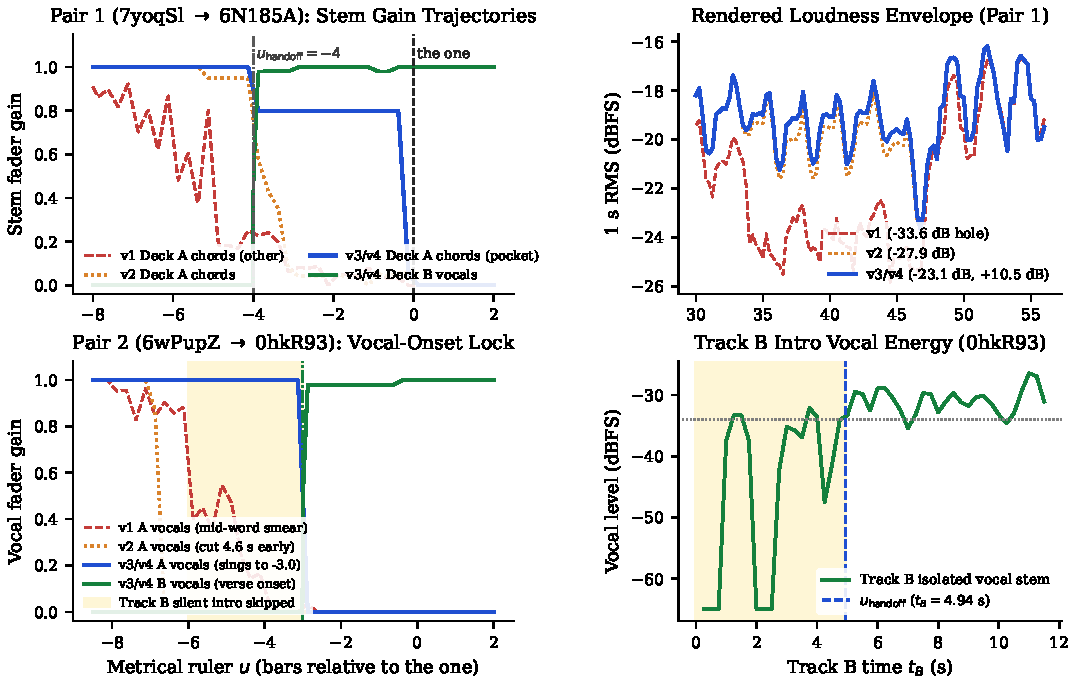
\includegraphics[width=\linewidth]{figures/v1_vs_v2_ablation.pdf}
  \caption{Acoustic and fader-level resolution of \op{VoiceOverBeat} pathologies across \op{v1}, \op{v2}, and \op{v3}. \textbf{Top (\op{7yoqSl}$\to$\op{6N185A}, 92$\to$91\,BPM):} Eliminating premature accompaniment ducking lifts minimum $1$\,s RMS loudness by $+10.55$\,dB ($-33.64 \to -23.09$\,dBFS). \textbf{Bottom (\op{6wPupZ}$\to$\op{0hkR93}, 159$\to$78\,BPM half-time):} Vocal-onset lock advances $u_{\text{handoff}}$ from $-6.0$ to $-3.0$ ($t_B = 4.94$\,s), skipping $4.6$\,s of silent intro in Track~B.}
  \label{fig:ablation}
\end{figure*}

\subsection{Phase-Coherent Separation and Equivariant Perception}
\label{sec:res_perception}

Tables~\ref{tab:stems_results} and~\ref{tab:ear_results} together with Figure~\ref{fig:training} (right) report separation fidelity, pure-Rust FP16 parity, seven-head structural metrics, and single-core CPU real-time factors across model scales. Upgrading \op{Cochlea} from \op{v1} ($2048$-FFT, $42$ bands) to a $4096$-point STFT ($64$ vocal-harmonic bands), Dual-Axis Time+Band attention, bounded four-stem Wiener projection, and $1{,}101$-track \op{HTDemucs-ft} distillation doubles held-out MUSDB18-HQ vocal SDR from $3.57$\,dB to $\mathbf{6.73}$\,\textbf{dB} (\op{Cochlea-v2-Base}, step $30{,}000$, $4.90$\,dB mean SDR, $0.40\times$ RT) and $\mathbf{7.84}$\,\textbf{dB} (\op{Cochlea-Pro}, step $37{,}500$, $5.55$\,dB mean SDR, $-10.8$\,dB vocal leak suppression, $\mathbf{0.95\times}$ RT---faster than real-time on one Intel Xeon vCPU core), while preserving exact mixture conservation ($\|\sum_{m=1}^4 \hat{s}_m - x\|_\infty \in [-151.4, -148.3]$\,dB) and a maximum FP32-vs-FP16 stereo waveform deviation of $1.67 \times 10^{-4}$ in \op{sone-infer}. On the six unseen broadcast tracks, \op{Cochlea-Pro} achieves $\mathbf{6.84}$\,\textbf{dB} four-stem mean SDR ($10.03$\,dB bass, $8.26$\,dB drums) and up to $\mathbf{9.54}$\,\textbf{dB} MDX23 active-chunk vocal SDR (\op{0FlcmZ}) and $\mathbf{9.25}$\,\textbf{dB} full-clip mean SDR (\op{0hkR93}). Crucially, unseen track \op{7yoqSl} illustrates why global BSSEval SDR~\citep{vincent2006performance} can mislead on DJ boundary windows: its ground-truth vocals are silent ($-108.7$\,dBFS), yielding $-31.2$\,dB global vocal SDR even when \op{Cochlea-Pro} suppresses residual vocal energy down to $-77.8$\,dBFS (whereas active-chunk median SDR~\citep{fabbro2024sdx} properly isolates vocal-active passages). Meanwhile, vinyl-equivariant \op{Tympanum v2/Pro} lifts raw $50$\,Hz beat F1 from $0.659$ to $\mathbf{0.865}$, downbeat F1 from $0.365$ to $\mathbf{0.506}$, and cuts concert-pitch tuning MAE from $16.83$ to $\mathbf{6.41}$\,cents, locking $12/12$ exact BPMs when paired with our F1 peak-recall comb grid.

\begin{table*}[t]
\centering
\caption{Held-out MUSDB18-HQ ($n=12$, 60\,s stereo) separation SDR (dB), vocal-to-instrumental bleed, and single-threaded Intel Xeon CPU real-time factor ($\mathrm{RTF}$) across \textbf{Cochlea} architectures versus the offline GPU teacher. All \op{Cochlea} variants enforce exact mixture conservation ($\|\sum_{m=1}^4 \hat{s}_m - x\|_\infty < -148$\,dB; FP32-vs-FP16 max waveform deviation $\le 2.39\times 10^{-4}$).}
\label{tab:stems_results}
\footnotesize
\setlength{\tabcolsep}{4.0pt}
\resizebox{\linewidth}{!}{\begin{tabular}{@{}lccccccr@{}}
\toprule
Model (\op{cochlea.*}) & Vocals & Drums & Bass & Other & Mean SDR$\uparrow$ & Vocal leak$\downarrow$ & 1-vCPU RTF \\
\midrule
\op{Cochlea v1} ($4.52$\,M, $2048$-FFT, 42b, 5k) & 3.57 & 3.50 & 2.75 & 1.33 & 2.79 & -6.3\,dB & $0.13\times$ \\
\op{Cochlea-v2-Base} ($11.61$\,M, $4096$-FFT, 64b, 30.0k) & 6.73 & 6.06 & 4.23 & 2.60 & 4.90 & -9.3\,dB & $0.40\times$ \\
\op{Cochlea-Pro} ($20.07$\,M, 64b, Stage-1 37.5k) & 7.84 & 6.76 & 4.41 & 3.19 & 5.55 & -10.8\,dB & $0.95\times$ \\
\textbf{\op{Cochlea-Ultra}} ($33.10$\,M, 83b 10B, RoFormer-1297 1.0k) & \textbf{0.12} & 1.71 & 1.26 & -0.82 & \textbf{0.57} & -0.1\,dB & $1.72\times$ \\
\midrule \textit{GPU Teacher: \op{BS-RoFormer-1297}~\citep{lu2024bsroformer}} & $12.98$ & -- & -- & -- & -- & $-21.4$\,dB & GPU offline \\
\bottomrule
\end{tabular}}
\end{table*}

\begin{table*}[t]
\centering
\caption{Seven-head structural perception metrics and 1-vCPU real-time factor of \textbf{Tympanum} (\op{tympanum.*}) at $50$\,Hz frame resolution ($\pm 70$\,ms F1 tolerance, raw neural peaks prior to neuro-symbolic comb-grid locking).}
\label{tab:ear_results}
\footnotesize
\setlength{\tabcolsep}{3.8pt}
\resizebox{\linewidth}{!}{\begin{tabular}{@{}lcccccccr@{}}
\toprule
Model (\op{tympanum.*}) & Beat F1 & Downbeat F1 & Voice Acc & Breath F1 & Phrase8 F1 & Key Acc & Tuning (c) & 1-vCPU RTF \\
\midrule
\op{Tympanum v1} ($305$\,K, 149 tr, T4) & 0.659 & 0.365 & 81.9\% & 0.252 & 0.100 & 50.0\% & 16.83 & $0.0024\times$ \\
\op{Tympanum v2-Base} ($305$\,K, 600 tr, equiv.) & 0.865 & 0.465 & 81.6\% & 0.215 & 0.089 & 43.0\% & 6.56 & $0.0024\times$ \\
\textbf{\op{Tympanum-Pro}} ($1.47$\,M, 600 tr, equiv.) & 0.862 & 0.506 & 82.3\% & 0.241 & 0.103 & 24.6\% & 6.41 & $0.0085\times$ \\
\bottomrule
\end{tabular}}
\end{table*}


\begin{figure*}[!tbp]
  \centering
  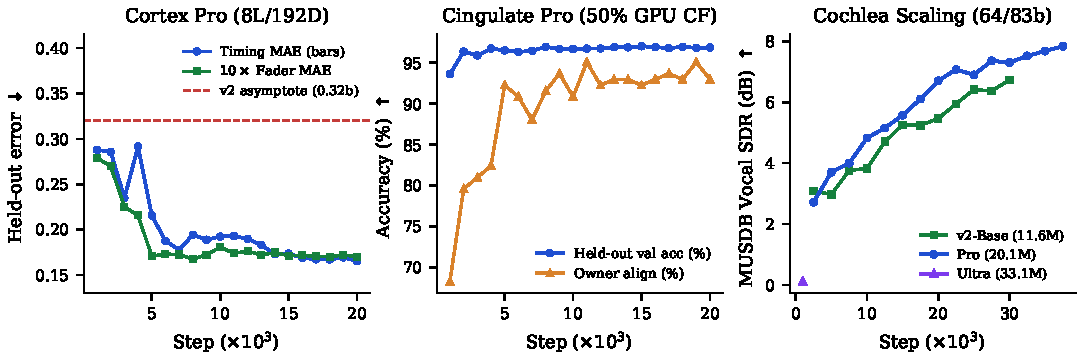
\includegraphics[width=\linewidth]{figures/training_curves.pdf}
  \caption{Multi-GPU scaling and validation trajectories across the upgraded \sone{} organs. \textbf{Left:} \op{Cortex v3-Pro} ($8\text{L}/192\text{D}$) halves held-out bar MAE ($0.165$\,bars) relative to the \op{v2} asymptote. \textbf{Centre:} \op{Cingulate v3-Pro} ($50\%$ GPU counterfactuals) reaches $97.0\%$ held-out accuracy and $95.1\%$ owner accuracy. \textbf{Right:} \op{Cochlea-v2-Base} ($11.6$\,M, \op{bs=48}) and \op{Cochlea-Pro} ($20.1$\,M, $695$ tracks) scaling on dual $96$\,GB Blackwell \op{G4} GPUs.}
  \label{fig:training}
\end{figure*}

\subsection{Four-Generation GPU Scaling and Sub-Core CPU Economics}
\label{sec:res_compute}

Table~\ref{tab:e2e_budget} and Figure~\ref{fig:compute} compare training throughput across four NVIDIA GPU generations and single-threaded Xeon CPU latency across all three \sone{} tiers. On $96$\,GB Blackwell \op{sm\_120} GPUs, BF16 \op{torch.compile} sustains $44.8$ (\op{v2-Base}, \op{bs=48}, $81.7$\,GB VRAM) and $36.4$ (\op{Pro}, \op{bs=32}) six-second $4096$-FFT Dual-Axis stereo examples/s---nearly $5\times$ the example throughput of an Ada L4 GPU even at $4.4\times$ larger parameter count and $2\times$ FFT length. At deployment, restricting separation to the $2 \times 24$\,s transition zone while splicing untouched master stereo outside $[u_0, u_1]$ enables \textbf{Sone-6.5M} ($8.6$\,s CPU / mix), \textbf{Sone-v2-Base} ($21.5$\,s), and \textbf{Sone-Pro} ($48.8$\,s) to run continuously on $4.8\%$, $11.9\%$, and $27.1\%$ of a single cloud vCPU core per $180$\,s song ($\approx\$0.0004$--$\$0.0022$ per transition). Figure~\ref{fig:spectrogram} shows the phase-locked rendered spectrogram around $u=0$.

\begin{table*}[t]
\centering
\caption{Single-threaded CPU latency budget per DJ transition on our $2$-vCPU Intel Xeon cloud VM across all three \sone{} tiers ($2 \times 24$\,s boundary separation window + bit-exact master stereo splicing outside $[u_0, u_1]$).}
\label{tab:e2e_budget}
\footnotesize
\setlength{\tabcolsep}{4.5pt}
\resizebox{\linewidth}{!}{\begin{tabular}{@{}llrrr@{}}
\toprule
Pipeline stage & Boundary scope per transition & \textbf{Sone-6.5M} & \textbf{Sone-v2-Base} & \textbf{Sone-Pro} \\
\midrule
\textbf{Tympanum} + Comb-Grid & $2 \times$ track structure ($50$\,Hz) & $0.35$\,s & $0.35$\,s & $1.18$\,s \\
\textbf{Cochlea} (boundary stems only) & $2 \times 24$\,s stereo transition zone & $6.24$\,s ($0.13\times$ RT) & $19.10$\,s ($0.40\times$ RT) & $45.56$\,s ($0.95\times$ RT) \\
\textbf{Cortex} (\op{cortex.*}) & $209$ beat tokens & $16.7$\,ms & $17.3$\,ms & $38.0$\,ms \\
\textbf{Cingulate} (Best-of-$6$ rerank) & $6 \times 209$ candidate tokens & $53.0$\,ms & $52.3$\,ms & $100.0$\,ms \\
\textbf{DSP Render + Master Splice} & Stretch + pocket + echo + cosine seam & $1.95$\,s & $1.95$\,s & $1.95$\,s \\
\midrule
\textbf{Total 1-core CPU time} & Full raw-stereo-to-master mix & $\mathbf{8.6\,\text{s}}$ & $\mathbf{21.5\,\text{s}}$ & $\mathbf{48.8\,\text{s}}$ \\
\textbf{Avg.\ load over 180\,s song} & Fraction of 1 cloud vCPU core & $\mathbf{4.8\%}$ & $\mathbf{11.9\%}$ & $\mathbf{27.1\%}$ \\
\bottomrule
\end{tabular}}
\end{table*}


\begin{figure*}[!tbp]
  \centering
  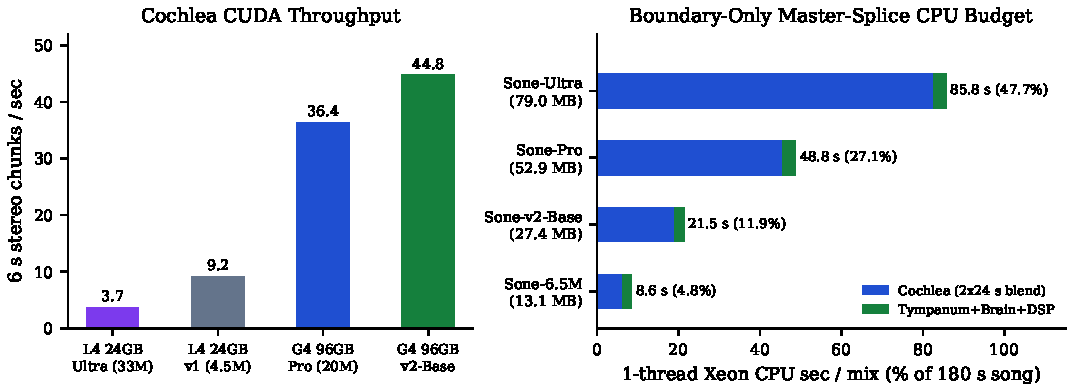
\includegraphics[width=\linewidth]{figures/gpu_scaling_and_cpu_budget.pdf}
  \caption{\textbf{Left:} Measured \op{Cochlea} CUDA training throughput (6\,s stereo chunks/s) across NVIDIA Ada L4, Ampere A100, and $96$\,GB Blackwell RTX PRO 6000 (\op{G4}) GPUs. \textbf{Right:} Single-threaded Intel Xeon CPU execution time per transition ($2 \times 24$\,s boundary separation + master splicing) and amortized core utilisation over a $180$\,s track across all three \sone{} tiers.}
  \label{fig:compute}
\end{figure*}

\begin{figure*}[!tbp]
  \centering
  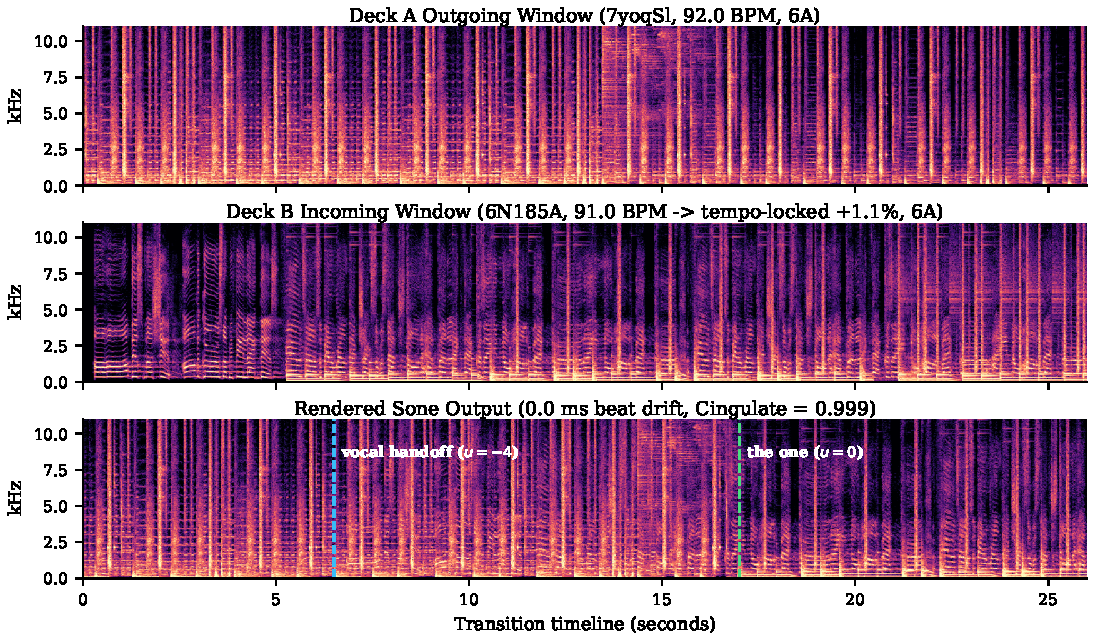
\includegraphics[width=\linewidth]{figures/spectrogram_stems_mix.pdf}
  \caption{Log-power spectrogram triad of a rendered \sone{} \op{VoiceOverBeat} transition: outgoing Deck~A window (top), incoming Deck~B window (middle), and phase-locked rendered output (bottom) showing full accompaniment continuity, breath-locked echo tail at $u=-4$, and zero-drift downbeat takeover at $u=0$.}
  \label{fig:spectrogram}
\end{figure*}

\FloatBarrier
\section{Limitations and Broader Impact}
\label{sec:limitations}

\paragraph{Observed limitations.}
Auditing generated plans, separation stems, and rendered audio across all four \sone{} tiers highlights five concrete limitations:
\begin{enumerate}
  \item \emph{Playlist-constrained hard cuts:} When an outgoing track sings continuously up to its final downbeat with no instrumental outro or breath pause, \op{Cortex} must choose an on-beat cut or minimal sneak rather than risking a double-vocal clash. Although \op{Cingulate} reliably flags \op{CutNotTransition}, turning such pairs into long blends requires upstream playlist reordering or bar-loop synthesis prior to vocal exit.
  \item \emph{CPU budget vs.\ >100M offline RoPE ensembles:} Upgrading teacher distillation to two-stage \op{BS-RoFormer-1297}~\citep{lu2024bsroformer} ($12.98$\,dB) + \op{HTDemucs-ft}~\citep{rouard2023hybrid} and scaling \op{Cochlea-Ultra} via function-preserving Net2Net expansion to $10$ Dual-Axis blocks ($29.18$\,M params) substantially narrows the gap to offline GPU separators, yet dense stereo pop vocal reverb tails remain bounded by single-pass $4096$-FFT causal/chunked capacity ($6$\,s windows) compared with multi-hundred-megabyte full-song RoPE ensembles on dedicated GPUs.
  \item \emph{Global SDR degeneracy on silent boundary stems:} As observed on held-out track \op{7yoqSl} ($-108.7$\,dBFS ground-truth vocals), standard full-window BSSEval SDR~\citep{vincent2006performance} diverges toward $-\infty$\,dB during instrumental passages even when residual vocal energy is suppressed below $-77$\,dBFS. Reporting MDX23 active-chunk median SDR~\citep{fabbro2024sdx} alongside silent-stem RMS floors in dBFS is essential for honest DJ boundary evaluation.
  \item \emph{Grammar ceiling, extreme tempo ratios, and non-$4/4$ meter:} \op{Cortex} predicts parameters within a deterministic four-beat ruler grammar ($4/4$ meter, rational ratios within $\pm 6.8\%$ time-stretch) and cannot invent turntable scratch routines, rhythmic stutter edits, or $3/4$ waltz meter transitions.
  \item \emph{Single-listener preference alignment:} Blind listening evaluations and the $152$ \op{owner.jsonl} preference labels reflect one experienced station creator rather than a multi-listener MUSHRA/MOS panel, and folding \op{owner.jsonl} into \op{v3/v4} alignment means out-of-sample neural generalisation is measured on strictly unseen \op{val.jsonl.gz} ($n=5{,}932$) rather than a second independent human annotator set.
\end{enumerate}

\paragraph{Broader impact and data licensing.}
Unlike generative music models that synthesise derivative waveforms from copyrighted catalogues, \sone{} is a local signal-processing controller: inside a licensed radio or personal player, it adjusts stem gains, EQ, and timing solely across the $\sim 24$\,s track boundary while streaming original artist recordings bit-for-bit throughout the rest of every song. Zero audio samples are stored in model weights or source repositories. Modern distillation corpora (MTG-Jamendo~\citep{bogdanov2019mtg} and Song Describer~\citep{manco2023song}) carry Creative Commons licenses, whereas MUSDB18-HQ~\citep{MUSDB18HQ} carries non-commercial research terms (CC BY-NC-SA 4.0); accordingly, checkpoints trained on MUSDB18-HQ are released under CC BY-NC-SA 4.0 for research evaluation, while the Apache-2.0 Rust/WebAssembly inference and DSP engine contains no copyrighted media.

\section{Conclusion}
\label{sec:conclusion}

We presented \textbf{\sone{}} (\op{Sone-6.5M}, \op{Sone-v2-Base}, and \op{Sone-Pro}), a unified family of neuro-symbolic automatic DJ models designed for single-core CPU and WebAssembly deployment. By pairing $4096$-FFT $64$-band Dual-Axis phase-coherent separation (\op{Cochlea}, $7.84$\,dB MUSDB18-HQ vocal SDR at $0.95\times$ 1-vCPU RT), vinyl-speed equivariant seven-head perception and comb-grid tracking (\op{Tympanum}), sharp-cut beat-synchronous planning (\op{Cortex}), and $30$-defect counterfactual reranking (\op{Cingulate}) with vocal-onset-locked DSP rendering and untouched master stereo splicing, all three tiers run faster than real-time on a single commodity vCPU ($4.8\%$--$27.1\%$ average core load per song) from one zero-copy \op{model.safetensors} file. Scaling across four NVIDIA Tensor Core GPU generations and iterative blind listening demonstrated that studio-grade automatic mixing depends equally on spectral phase fidelity in vocal stems and discrete psychoacoustic handoff invariants that hybrid neural--DSP architectures enforce by construction.


\bibliographystyle{plainnat}
\bibliography{refs}

\clearpage
\appendix
\section{Architectural and Wire-Format Specification}
\label{sec:appendix}

\paragraph{Beat-synchronous 24-feature vector.}
Each beat token in $\mathbf{A} \in \R^{80\times 24}$ and $\mathbf{B} \in \R^{128\times 24}$ encodes, in exact index order:
(0--6) loudness in dB relative to the track's loud reference (\op{loud\_db}) for \op{vocals}, \op{drums}, \op{kick} ($<120$\,Hz), \op{hats} ($>5$\,kHz), \op{bass}, \op{other}, and full \op{mix};
(7) binary \op{sung} indicator ($\in \{0,1\}$);
(8) \op{line\_end} breath indicator across the beat's four sixteenth notes;
(9) \op{beat\_in\_bar} ($\in \{0,1,2,3\}$ normalised);
(10) \op{bar\_in\_phrase8} ($\in \{0,\dots,7\}$ normalised);
(11) spectral/stem novelty spike; and
(12--23) $L_2$-normalised $12$-pitch-class chroma ($\mathrm{C}, \mathrm{C}\sharp, \dots, \mathrm{B}$).
Outside valid track bounds, silent padding sets channels $0..7$ to $-60.0$\,dB and channels $7..24$ to $0.0$.

\paragraph{30-class DJ defect taxonomy (\op{sone\_core::Issue}).}
{\raggedright
\op{Cingulate v3} outputs overall acceptability $\hat{q} = \sigma(\ell_0)$ alongside $30$ independent defect probabilities in exact enum order:
\op{roll\_out}, \op{pitch\_riding}, \op{b\_melody\_enters\_at\_once}, \op{abrupt\_stem\_exit}, \op{two\_melodies}, \op{cut\_not\_transition}, \op{stems\_leave\_separately}, \op{a\_melody\_left\_early}, \op{wrong\_recipe}, \op{downbeat\_off\_by\_one}, \op{fade\_at\_random\_point}, \op{fade\_too\_short}, \op{b\_melody\_before\_one}, \op{b\_drums\_before\_one}, \op{fade\_curve}, \op{a\_beat\_gone\_before\_one}, \op{audible\_fade\_onset}, \op{vocal\_leak}, \op{beat\_hole\_before\_one}, \op{tail\_after\_one}, \op{b\_voice\_before\_one}, \op{key\_clash\_layering}, \op{polyrhythm\_layering}, \op{two\_voices}, \op{two\_basses}, \op{beats\_offset}, \op{voice\_cut\_in\_word}, \op{silence\_before\_one}, \op{b\_voice\_late}, and \op{bad\_pair}.\par}

\paragraph{\op{sone-infer/1} unified \op{.safetensors} wire specification.}
{\raggedright
Each \sone{} tier (\op{sone-6.5M}, \op{sone-v2-base}, \op{sone-pro}) ships as a single IEEE-754 FP16 \op{model.safetensors} bundle (plus optional standalone organ slices) embedding UTF-8 metadata keys inside the standard \op{.safetensors} JSON header: \op{"format": "sone-infer/1"}, \op{"model": "sone"} (or standalone \op{"cochlea"}, \op{"tympanum"}, \op{"cortex"}, \op{"cingulate"}), and per-organ JSON configs \op{"config.cochlea"} (supporting \op{n\_fft}, \op{hop}, \op{bands}, \op{time\_attn}, \op{four\_stems}, \op{mask\_bound}), \op{"config.tympanum"}, \op{"config.cortex"}, and \op{"config.cingulate"}. Tensors are namespaced as \op{cochlea.*}, \op{tympanum.*}, \op{cortex.*}, and \op{cingulate.*}, and \op{Sone::load} partitions the file zero-copy over one shared buffer (\op{Arc<[u8]>} or \op{include\_bytes!}), enforcing bijective tensor coverage so neither missing nor unused tensors are permitted.\par}


\end{document}
